\documentclass[a4paper,12pt]{article}
\usepackage[utf8]{inputenc}
\usepackage{graphicx}
\usepackage[margin=1in]{geometry}
\usepackage{titling}
\usepackage{fancyhdr} % header and footer
\usepackage{everypage}
\usepackage{hyperref}
\graphicspath{ {./images} }

\hypersetup{
    colorlinks=false,
}

\fancypagestyle{plain}{ 
    \fancyhf{}
    \renewcommand{\headrulewidth}{0pt}
    \renewcommand{\footrulewidth}{0pt}
}

\fancyhf{}
\fancyhead[L]{
\includegraphics[width=0.3\textwidth]{logo_ipl.png}}
\fancyhead[R]{
    \small Licenciatura em Eng. Informática\\
    Ano Letivo 2024/2025\\
    Sistemas Gráficos e Interação -- Projeto
}
\setlength{\headsep}{2cm}
\renewcommand{\headrulewidth}{0pt}
\renewcommand{\contentsname}{Índice}

\fancyfoot[R]{\thepage} 
\setlength{\footskip}{0cm}
\pagestyle{fancy}

\begin{document}

\begin{titlepage}
\begin{center}
    
\includegraphics[width=0.5\textwidth]{logo_ipl.png}
\end{center}

\vspace{1cm}

\begin{center}
    \fboxsep=10pt
    \parbox[c][3cm][c]{0.8\textwidth}{
        \centering
        \textbf{\Large Relatório do Projeto de}\\[0.3cm]
        \textbf{\Large Interface web 3D}
    }
\end{center}

\vfill

\begin{center}
    \textbf{Licenciatura em Engenharia Informática}\\
    Sistemas Gráficos e Interação\\[0.5cm]
    \vspace{1cm}
    \textbf{Ano Letivo: 2024/2025}
\end{center}

\vfill

% Student information
\begin{center}
    \textbf{Estudantes:}\\[0.3cm]
    Marco Padeiro, 2231953\\
    Rodrigo Carreira, 2231952
\end{center}
\thispagestyle{plain}
\end{titlepage}

\newpage
\tableofcontents

\newpage
\section{Avaliação heurística}

\newpage
\section{Análise de Utilizadores e Tarefas}

\begin{center}
    \href{https://forms.gle/mGgTZJcjzfStsLvn6}{Link para o formulário}

    \vspace{0.3cm}
    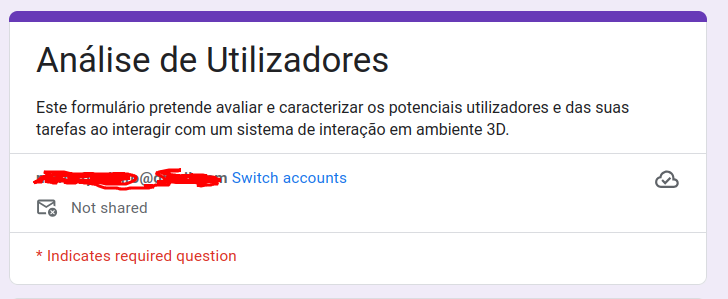
\includegraphics[width=0.75\textwidth]{form/intro_form.png}
    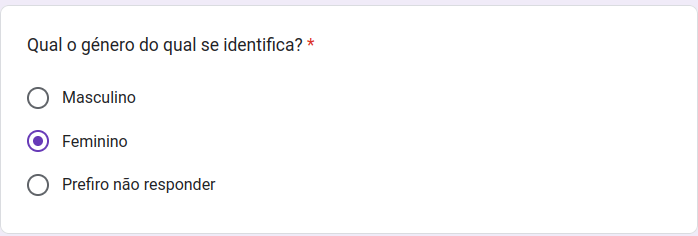
\includegraphics[width=0.75\textwidth]{form/01questao_genero.png}
    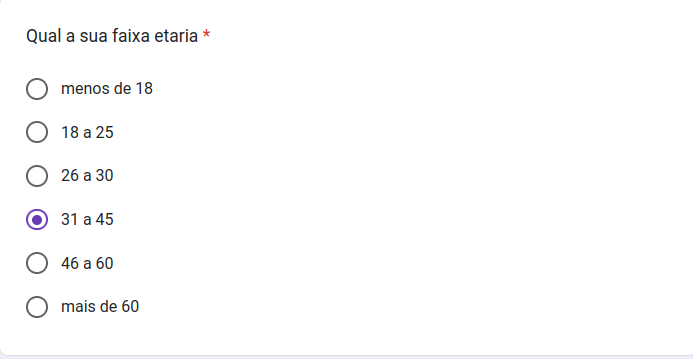
\includegraphics[width=0.75\textwidth]{form/02questao_idade.png}
    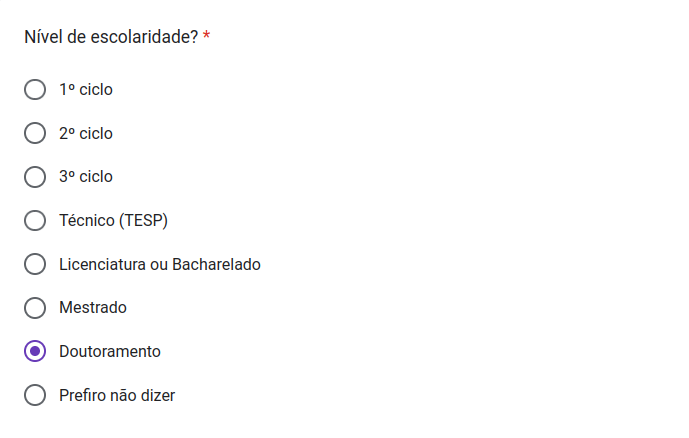
\includegraphics[width=0.75\textwidth]{form/03questao_escolaridade.png}
    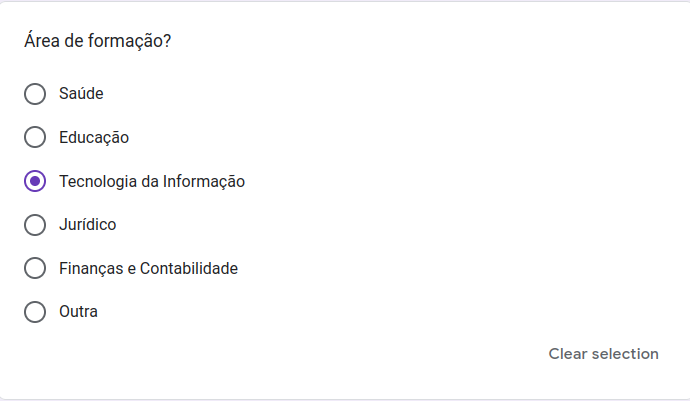
\includegraphics[width=0.75\textwidth]{form/04questao_formacao.png}
    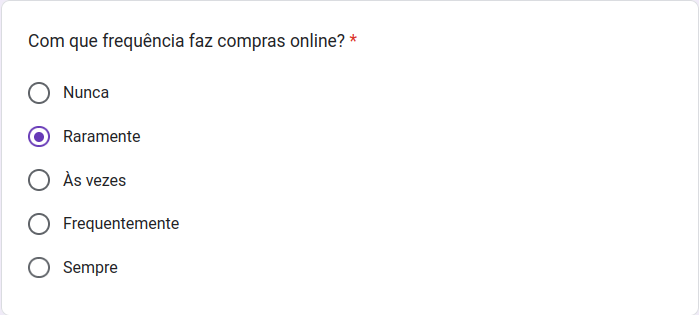
\includegraphics[width=0.75\textwidth]{form/05questao_comprasonline.png}
    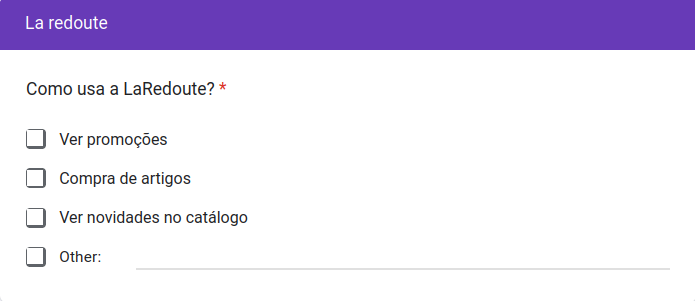
\includegraphics[width=0.75\textwidth]{form/06questao_usolaredoute.png}
    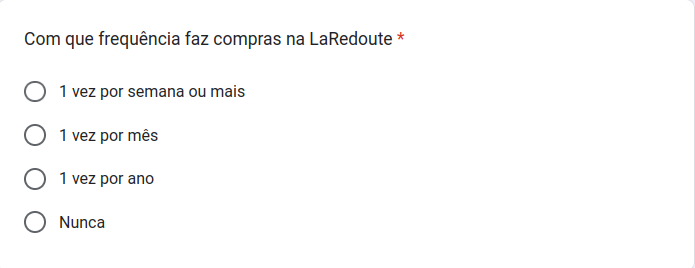
\includegraphics[width=0.75\textwidth]{form/07questao_frequencialaredoute.png}
    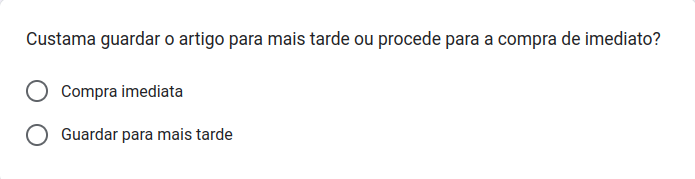
\includegraphics[width=0.75\textwidth]{form/08questao_guardarparatarde.png}
    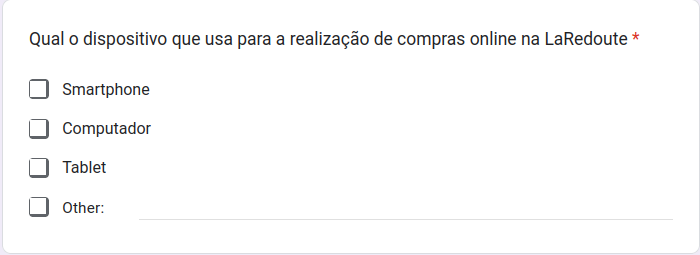
\includegraphics[width=0.75\textwidth]{form/09questao_dispositivocompra.png}
    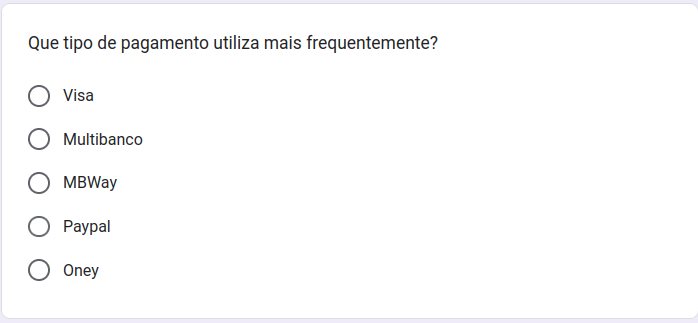
\includegraphics[width=0.75\textwidth]{form/10questao_metodopagamento.png}
    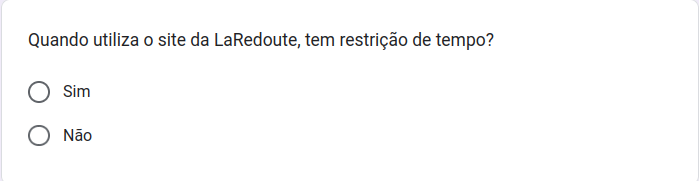
\includegraphics[width=0.75\textwidth]{form/11questao_restricaotempo.png}
    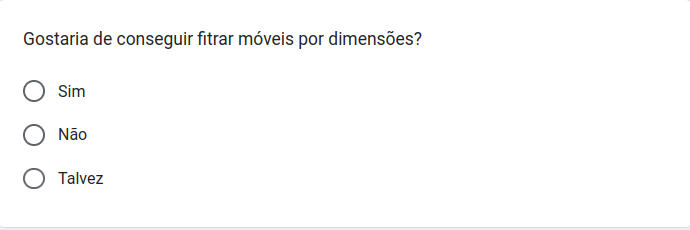
\includegraphics[width=0.75\textwidth]{form/12questao_filtrardimensoes.png}
    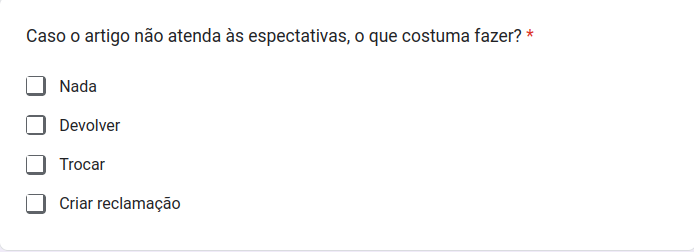
\includegraphics[width=0.75\textwidth]{form/13questao_expectativas.png}
    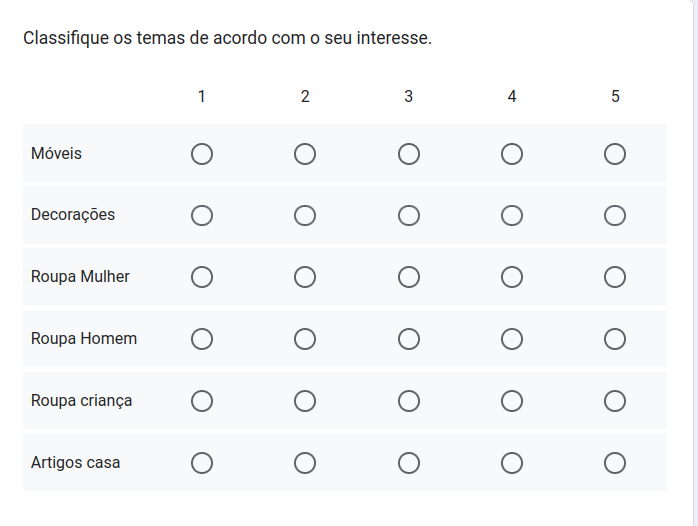
\includegraphics[width=0.75\textwidth]{form/14questao_temasinteresse.png}
    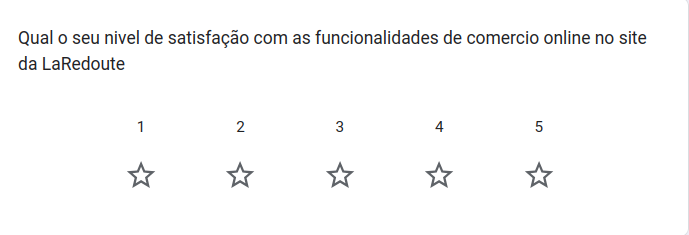
\includegraphics[width=0.75\textwidth]{form/15questao_satisfacao.png}
    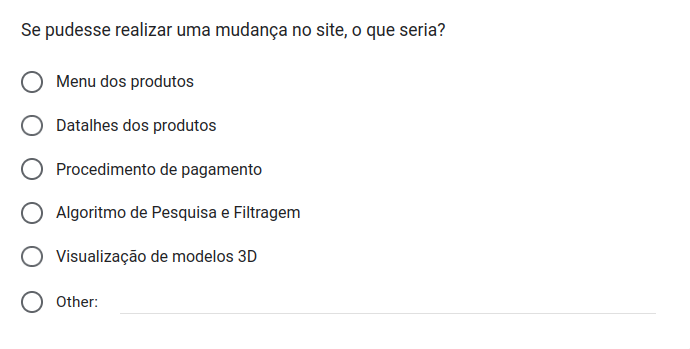
\includegraphics[width=0.75\textwidth]{form/16questao_mudancasite.png}
    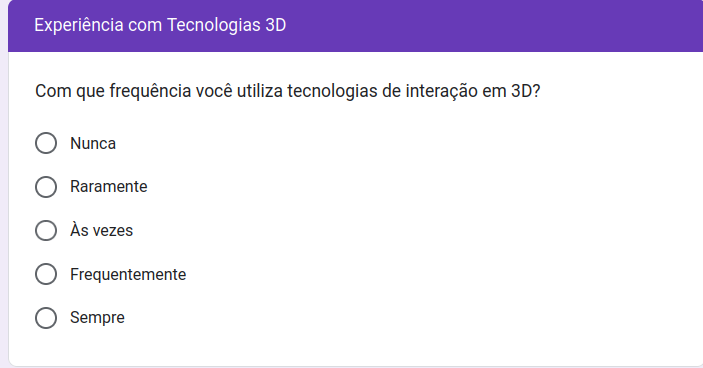
\includegraphics[width=0.75\textwidth]{form/17questao_frequencia3d.png}
    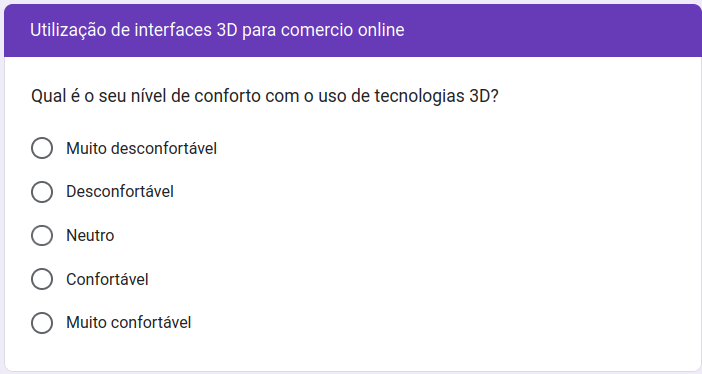
\includegraphics[width=0.75\textwidth]{form/18questao_conforto3d.png}
    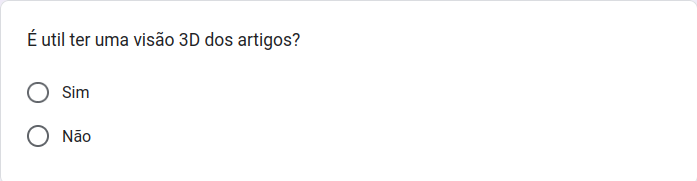
\includegraphics[width=0.75\textwidth]{form/19questao_visao3d.png}
    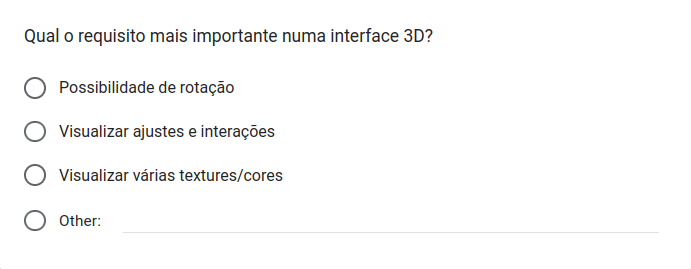
\includegraphics[width=0.75\textwidth]{form/20questao_requisito3d.png}
\end{center}

\newpage
\section{Requisitos funcionais}
    Permitir que o utilizador possa:
    \begin{itemize}
        \item Escolher diferentes textures
        \item Efetuar rotações ao objeto 3D
        \item Visualizar uma animação que muda o ângulo do braço do candeeiro
    \end{itemize}

\newpage
\section{Avaliação da Usabilidade do Sistema}

\newpage
\section{Análise/Discussão dos resultados}


\end{document}
